%        File: test.tex
%     Created: Thu Apr 21 03:00 PM 2011 C
% Last Change: Thu Apr 21 03:00 PM 2011 C
%

\documentclass[a4paper]{article}

\usepackage{amsmath}
\usepackage{graphicx}

\begin{document}

\section{Problem}
We have sampled a set of $n$ individuals $I$ from the general population. For each individual $i \in I$ we have gathered some information:
\begin{itemize}
  \item A matrix $S$ of size $n \times m$ that contains the set of sampled SNPs for each individual. Each element $s_{i,j} \in \{0,1,2\}$ describes the number of alleles for SNP $j$ for individual $i$.
  \item A matrix $R$ of risk factors of size $n \times k$. Each element $r_{i,j} \in \{0,1\}$ describes the risk factor $j$ for individual $i$.
  \item A vector $c$ of length $n$ that classifies each individual $i$ as healthy ($c_i = 0$) or sick ($c_i = 1$).
\end{itemize}
The problem is given this information find a set of predictors, in terms of SNPs and risk factors, that effectively predicts whether an individual is healthy or sick.
\section{Method}
This section describes the general outline of the method. As a first step we will only consider one SNP at a time. This is done for simplicity and there is no loss of generality. We can always include several SNPs at the same time limited by computational complexity. The general method outline for creating a predictor for a single SNP is given below.
\begin{enumerate}
  \item Generate all possible predictors for $1$ SNP and $k$ risk factors.
  \item Order predictors by true positives divided by false positives.
  \item Generate a ROC curve by stepwise including a predictor in the order specified above.
  \item Evaluate each set of predictors by the corresponding ROC curve.
\end{enumerate}
Once we have a predictor set for each SNP, we can use cross model validation to find the best predictor sets.

\subsection{Generate predictors}
This section will describe how to generate a set of predictors. In short we will evaluate all possible predictors and join the best ones to form a better predictor. To simplify the notation, let us from now on assume that $m = 1$ so that $S$ is reduced to a vector $s$ where $s_i$ denotes the number of alleles of the SNP for individual $i$.

The predictors that we will use are on the form $(s, r_1, \cdots, r_k)$, this predictor will classify an individual as sick if it has $s$ alleles of the specific SNP and the risk factors are equal to $r_1$, $r_2$, \ldots $r_k$. For example, if we have the individuals $\{(2,2,1,0),(0,1,0,1),(2,1,0,1),(2,2,0,1)\}$ with $2$ SNPs and $2$ risk factors. A predictor $p = (2,0,1)$ for the first SNP and two risk factors will classify $(2,1,0,1)$ and $(2,2,0,1)$ as sick.

We begin by creating the set of all predictors $P = \{0,1,2\}\times\{0,1\}^k$, which contains all possible assignments of a single SNP and the $k$ risk factors. This size of this set grows exponentially with $k$, $|P| = 3 \cdot 2^k$, so we can only handle small values of $k$. The set of all predictors implies a partition $\{A_1, A_2, \cdots, A_{|P|}\}$ on the set of individuals $I$. Let $snp(p)$ project the SNP from a predictor $p \in P$, $rf(p)$ project the risk factor vector from a predictor $p \in P$, and $P_i$ denote the $i$:th predictor (in any order) then $A_i = \{ j \in I | snp(P_i) = s_j, rf(P_i) = r_j \}$ contains the individuals matched by predictor $P_i$.
\subsection{Generate ROC curve}
Now lets define two measures:
\begin{itemize}
  \item The number of healthy individuals in $A_i$: $x_i = |\{j \in A_i | c_j = 0\}|$. These are the false positives for predictor $P_i$.
  \item The number of sick individuals in $A_i$: $y_i = |\{j \in A_i | c_j = 1\}|$. Similarly, these are the true positives for predictor $P_i$.
\end{itemize}
We will now use $x_i$ and $y_i$ to generate a ROC curve. A ROC curve describes the relation between false positives ($x_i$) and true positives ($y_i$) when some threshold for classification is varied. In our case the threshold will be the number of predictors from $P$ that we include. We create a kind of summary predictor that matches if any of the underlying predictors match. The ROC curve then goes from $(0,0)$ where no predictor is used to $(1,1)$ where all predictors are included (and all individuals are classified as sick).

There are many ways to create such a summary predictor, in fact there are $|P|!=(3\cdot2^k)!$ ways so it is not feasible to try them all. Intuitively we want the ROC curve to rise as steeply as possible in the beginning in order to minimize the number of false positives. In terms of our predictors this means that the slope $\frac{y_i}{x_i}$ should be as steep as possible. The idea is therefore to begin with the predictor with the largest $\frac{y_i}{x_i}$, and extend the summary predictor with one more at a time ordered by the slope, and note the true positives and false positives in the ROC curve for each step. (Motivate here that the ROC curve constructed this way is optimal in some sense). Formally, let $P_{(i)}$ denote the ordered predictors where $P_{(1)}$ has the largest slope, then 
$$SP_1 = P_{(1)} \qquad \text{and} \qquad SP_i = SP_{i-1} \cup P_{(i)} \text{ for } i > 1.$$
The points in the ROC curve $(x'_n, y'_n)$ are then $x'_n = \sum_{i=1}^n x_{(i)}$ and analogously $y'_n = \sum_{i=1}^n y_{(i)}$. In figure \ref{fig:roc} you can see how a summary predictor $SP$ for $k=1$ generates a ROC curve.

\begin{figure}[h]
  \centering
  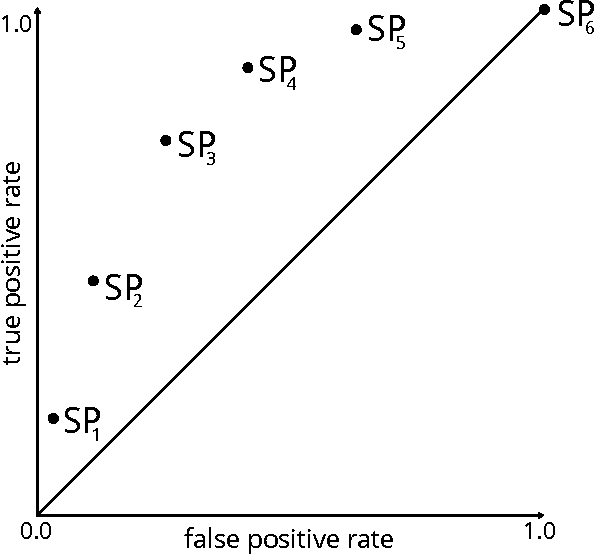
\includegraphics[scale=0.5]{graphics/roc}
  \caption{Illustrates how the increasing set of predictors in a summary predictor generates a ROC curve, for the case when we have a single risk factor.}\label{fig:roc}
\end{figure}

Finally, we can then use the ROC curve to determine which $SP_i$ to use as our ``optimal'' summary predictor.
\subsection{Cross Model Validation}
Above we have described to generate a summary predictor for a single SNP and a set of risk factors. We can perform the method above for each of our SNPs to get a larger set of summary predictors. We can then use cross model validation to determine which of these summary predictors that efficiently predict the disease.

\subsection{Time complexity}
I expect that a naive implementation will roughly have the time complexity $\mathcal{O}(m \cdot (2^k\cdot \log{2^k} + n))$. Since $m$ is fixed to around $200 000$, and $n$ is relatively small. It seems reasonable to run the algorithm as long $2^k$ is in the same order of magnitude as $n$, and the CMV step is similarly intensive.

\subsection{Notes}
Optimizing predictors with regards to $\frac{y_i}{x_i}$ is equivalent to the NP-complete problem of 0-1 programming.
\section{More ideas}
\begin{itemize}
  \item It might be an idea to use BIC instead of CMV but that will require a probabilistic model in order to calculate the likelihood term.
  \item If the total number of predictors becomes too large, it might be an idea to use an approximation algorithm for 0-1 programming, like a branch-and-bound algorithm. This means of course that we won't be able to calculate the whole ROC curve.
  \item Genetic algorithm for parameter search? Probably too expensive.
  \item Discretize continuous risk factors into several intervals e.g. \texttt{LOW}, \texttt{MEDIUM} and \texttt{HIGH} (make them qualitative features).
\end{itemize}

\end{document}
